\documentclass[tikz,border=5pt]{standalone}
\usepackage[american]{circuitikz}
\usepackage{graphicx}
\usetikzlibrary{calc}
\begin{document}
\begin{circuitikz}[american voltages,american currents,x=.60cm,y=.82cm,
 every node/.style={font=\sffamily\scriptsize},
 wire/.style={line width=.65pt},
 dot/.style={circ,fill=black,inner sep=1pt}]
% Compile scopes.tex first; it remains an independent oscilloscope artefact.
\IfFileExists{scopes.pdf}{\node[anchor=south west,inner sep=0] at (0,12) {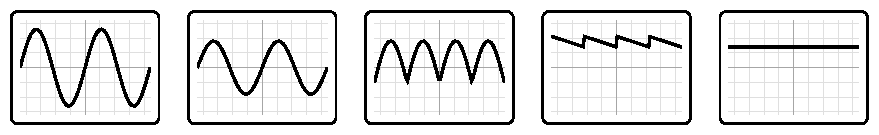
\includegraphics{scopes.pdf}};}{}
% Master rails
\draw[wire] (9,10)--(28,10) node[right]{VRAW};
\draw[wire] (25,5)--(28,5) node[right]{VOUT};
\draw[wire] (0,1)--(28,1) node[right]{GND};
% VAC and complete T1: primary left, isolated secondary right.
\draw (1,1) to[sV,l=VAC] (1,6);
\node[transformer core] (T1) at (3.3,4.0) {};
\draw (1,6)--(T1.A1);
\draw (1,1)|-(T1.A2);
\draw (T1.B1)--(5.8,6);
\draw (T1.B2)--(5.8,3);
\node[below] at (3.3,2.3) {T1};
\coordinate (VAC1) at (5.8,6);
\coordinate (VAC2) at (5.8,3);
\draw (5.8,6)--(VAC1) node[dot]{};
\draw (5.8,3)--(VAC2) node[dot]{};
% D1--D4 bridge, all interconnect paths Manhattan.
\coordinate (VP) at (9,8.2);
\coordinate (VN) at (9,1);
\draw (VAC1)|-(7.2,8.2) to[D,l=D1] (VP) node[dot]{};
\draw (VAC2)|-(7.2,7.0) to[D,l=D2] (8.5,7.0) |- (VP);
\draw (VN)--(8.5,1) to[D,l_=D3] (7.2,1) |- (VAC1);
\draw (VN)|-(8.5,2.2) to[D,l_=D4] (7.2,2.2) |- (VAC2);
\draw (VP)|-(9,10) node[dot]{};
\draw (VN)--(9,1) node[dot]{};
\draw (10.5,10) to[C,l=C1] (10.5,1);
% Reference and differential input pair
\draw (12,10) to[R,l=R3] (12,6.1) node[dot](REF){};
\draw (12,6.1) to[zD,l=DZ] (12,1);
\node[npn] (Q1) at (14.3,4.8) {};
\node[npn] (Q2) at (16.3,4.8) {};
\node[below] at (14.3,4.15) {Q1};
\node[below] at (16.3,4.15) {Q2};
\draw (Q1.B)-|(12,6.1);
\draw (Q1.E)|-(15.3,3.15) node[dot]{};
\draw (Q2.E)|-(15.3,3.15);
\draw (15.3,3.15) to[isource,l_=I1] (15.3,1);
% PNP mirror above differential pair
\node[pnp,xscale=-1] (Q3) at (14.3,8.1) {};
\node[pnp] (Q4) at (16.3,8.1) {};
\node[above] at (14.3,8.65) {Q3};
\node[above] at (16.3,8.65) {Q4};
\draw (Q3.E)|-(14.3,10);
\draw (Q4.E)|-(16.3,10);
\draw (Q3.B)-|(15.3,7.2)-|(Q4.B);
\draw (Q3.C)|-(15.3,7.2) node[dot]{};
\draw (Q1.C)|-(14.3,7.2)-|(15.3,7.2);
\coordinate (N2) at (16.3,7.2);
\draw (Q2.C)|-(N2) node[dot]{};
\draw (Q4.C)|-(N2);
% VAS and Miller. CC has its own vertical corridor.
\node[npn] (Q5) at (18.3,7.2) {};
\node[above] at (18.3,7.75) {Q5};
\draw (N2)--(Q5.B);
\draw (Q5.C)|-(18.3,10);
\coordinate (VAS) at (18.3,5.9);
\draw (Q5.E)|-(VAS) node[dot]{};
\draw (N2)-|(19.7,7.2) to[C,l=CC] (19.7,5.9)-|(VAS);
% Bias diodes and complementary driver
\draw (VAS) to[D,l=D5] (20.8,5.9) to[D,l=D6] (21.9,5.9);
\node[npn] (Q6) at (20.8,7.2) {};
\node[pnp] (Q7) at (21.9,7.2) {};
\node[above] at (20.8,7.75) {Q6};
\node[above] at (21.9,7.75) {Q7};
\draw (Q6.B)|-(20.8,5.9);
\draw (Q7.B)|-(21.9,5.9);
\draw (Q6.C)|-(20.8,10);
\draw (Q7.E)|-(21.9,10);
\coordinate (DRV) at (23,6.3);
\draw (Q6.E)-|(DRV) node[dot]{};
\draw (Q7.C)-|(DRV);
% Series NPN pass, sense resistor, and discrete limiter.
\node[npn] (Q8) at (24.3,8) {};
\node[above] at (24.3,8.55) {Q8};
\draw (24.3,10)|-(Q8.C);
\draw (DRV)-|(Q8.B);
\coordinate (SENSE) at (25.7,6.8);
\draw (Q8.E)|-(SENSE) node[dot]{};
\draw (SENSE) to[R,l=RSC] (25.7,5) node[dot]{};
\node[npn] (Q9) at (23.5,5.5) {};
\node[below] at (23.5,4.95) {Q9};
\draw (Q9.C)|-(DRV);
\draw (Q9.B)-|(SENSE);
\draw (Q9.E)-|(25.7,5);
% Divider and clean FB return corridor.
\draw (27,5) to[R,l=R1] (27,3.2) node[dot](FB){} to[R,l=R2] (27,1);
\draw (FB)-|(16.3,4.8)--(Q2.B);
\node[right] at (27,3.2) {FB};
% Explicit T-junctions.
\foreach \p in {(9,10),(12,6.1),(15.3,3.15),(15.3,7.2),(16.3,7.2),(18.3,5.9),(23,6.3),(25.7,6.8),(25.7,5),(27,3.2)}
 \node[dot] at \p {};
\end{circuitikz}
\end{document}
